\chapter{Análisis y Despliegue}

En este capítulo discutiremos cómo hemos llevado a cabo la evaluación de las herramientas disponibles en el estado del arte para la extracción de información en texto no estructurado de carácter médico.

Para ello se ha creado una web app disponible de forma muy accesible para que sea fácil ver el poder combinado de todas estas herramientas.

\section{Análisis de texto no estructurado}

Para el análisis y minería de texto no estructurado una de las técnicas más útiles es el \textbf{Named Entity Recognition (NER) Tagging}, es decir, el etiquetado de etiquetas. La idea es, dado un cuerpo de texto, extraer aquellas entidades que tengan un significado propio o relevante por sí solas. En nuestro contexto, esto corresponde, por ejemplo, a nombres de enfermedades, partes del cuerpo, medicamentos, entre otras. Un NER Tagger entrenado sería capaz de detectar dichas entidades en el texto y devolver una lista de las mismas, automatizando la extracción de información y haciéndolo muy rápido.

La librería SciSpacy \cite{neumann-etal-2019-scispacy} nos provee con una selección de NER Taggers preentrenados en diferentes corpus de caracter biomédico y los hace disponibles mediante la famosa librería Spacy \cite{spacy}, que se ha convertido en el estándar de la industria para el análisis del lenguaje natural.

Estos son los taggers que utilizaremos en nuestra aplicación, aunque la inclusión de algún otro más que pudiera ser interesante es trivial. 

\begin{itemize}
	\item \textbf{Med7} \cite{med7}: El Med7 es un NER entrenado en datos clínicos capaz de detectar 7 entidades diferentes: nombres de medicamentos, vía de administración del medicamento, frecuencia, dosis, cantidad, el formato (pastilla, polvos, etc), y el tiempo total de medicación. 
	\item \textbf{BC5CDR} \cite{bc5cdr}: Este tagger recibe su nombre del corpus en el que fue entrenado. Dicho corpus consta de 1500 artículos \textit{PubMed} con 4409 sustancias químicas etiquetadas, 5818 enfermedades y 3116 interacciones enfermedad-medicamento.
	\item \textbf{BIONLP13CG} \cite{BIONLP13CG}: De igual forma, este tagger recibe su nombre del corpus que lo origina. Este tagger se especializa más en términos genéticos, cánceres, órganos y compuestos químicos como aminoácidos o proteínas, ligeramente mejor adecuado para prescripciones quirúrgicas.
\end{itemize}

\begin{figure}[h]
	\centering
	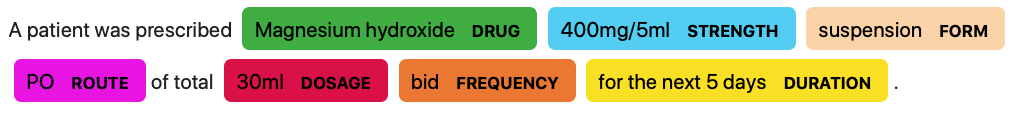
\includegraphics[width=.9\textwidth]{media/med7_example.png}
	\caption{Ejemplo del Med7 en acción. Vemos cómo las entidades se han reconocido en diferentes colores, haciendo la extracción de información mucho más eficiente. bid viene del latin \textit{bis in die}, que se traduce por dos veces al día. PO viene de \textit{Per os}, vía oral. Suspension hace referencia a una disolución en agua.}
	\label{fig:med7}
\end{figure}

En la figura \ref{fig:med7} vemos un ejemplo de cómo una de estas herramientas puede ayudar al análisis del texto, destacando con diferentes colores las entidades encontradas. Esto es, sin embargo, solo una aplicación de demostración. El verdadero poder reside en que dichas entidades están internamente representadas en forma de diccionario, asociando cada término encontrado en el texto con la entidad correspondiente. 

Estos diccionarios pueden anexarse y guardarse en la base de datos correspondiente, haciendo su búsqueda y análisis muchísimo más rápidos, además de habilitando comparativas que no serían posibles de otra forma.


\section{Despliegue de la aplicación}

Para hacer accesible todo el trabajo que se ha acometido, se ha elaborado una aplicación que permite hacer uso de todas las técnicas y herramientas discutidas a lo largo del documento. El framework utilizado ha sido \href{https://streamlit.io}{Streamlit}.

La aplicación permite generar comentarios utilizando el modelo generativo, y permite analizar dichos comentarios, así como importar desde distintas fuentes. La aplicación efectúa un pequeño análisis del texto y utiliza el tagger que el usuario seleccione.

Como vemos en las figuras \ref{fig:app-demo} y \ref{fig:analysis-comment}, la aplicación hace accesibles la generación y el análisis de los comentarios. Está pensada para que sea utilizada por desarrolladores de NER Taggers, o herramientas similares, de forma que fácilmente puedan incluir el modelo que están desarrollando y probarlo con los comentarios que nuestra aplicación genera.

Esto hace el desarrollo de dichos modelos más fácil para todos, contribuyendo a una mayor y mejor producción de herramientas de asistencia médica, clave para cualquier complejo hospitalario medianamente grande, ya que se manejan volúmenes de datos, a menudo, insostenibles.

La asistencia que estas herramientas ofrecen puede suponer una mejora en la calidad de la atención que cada paciente recibe, además de la reducción de carga cognitiva que los correspondientes profesionales deben soportar, mejorando la calidad de vida de ambas partes. Con todo ello, se apunta a una mejora del sistema médico del que disponemos, del que ya de por sí podemos estar orgullosos siendo uno de los mejores en el mundo.

\begin{figure}[h]
	\centering
	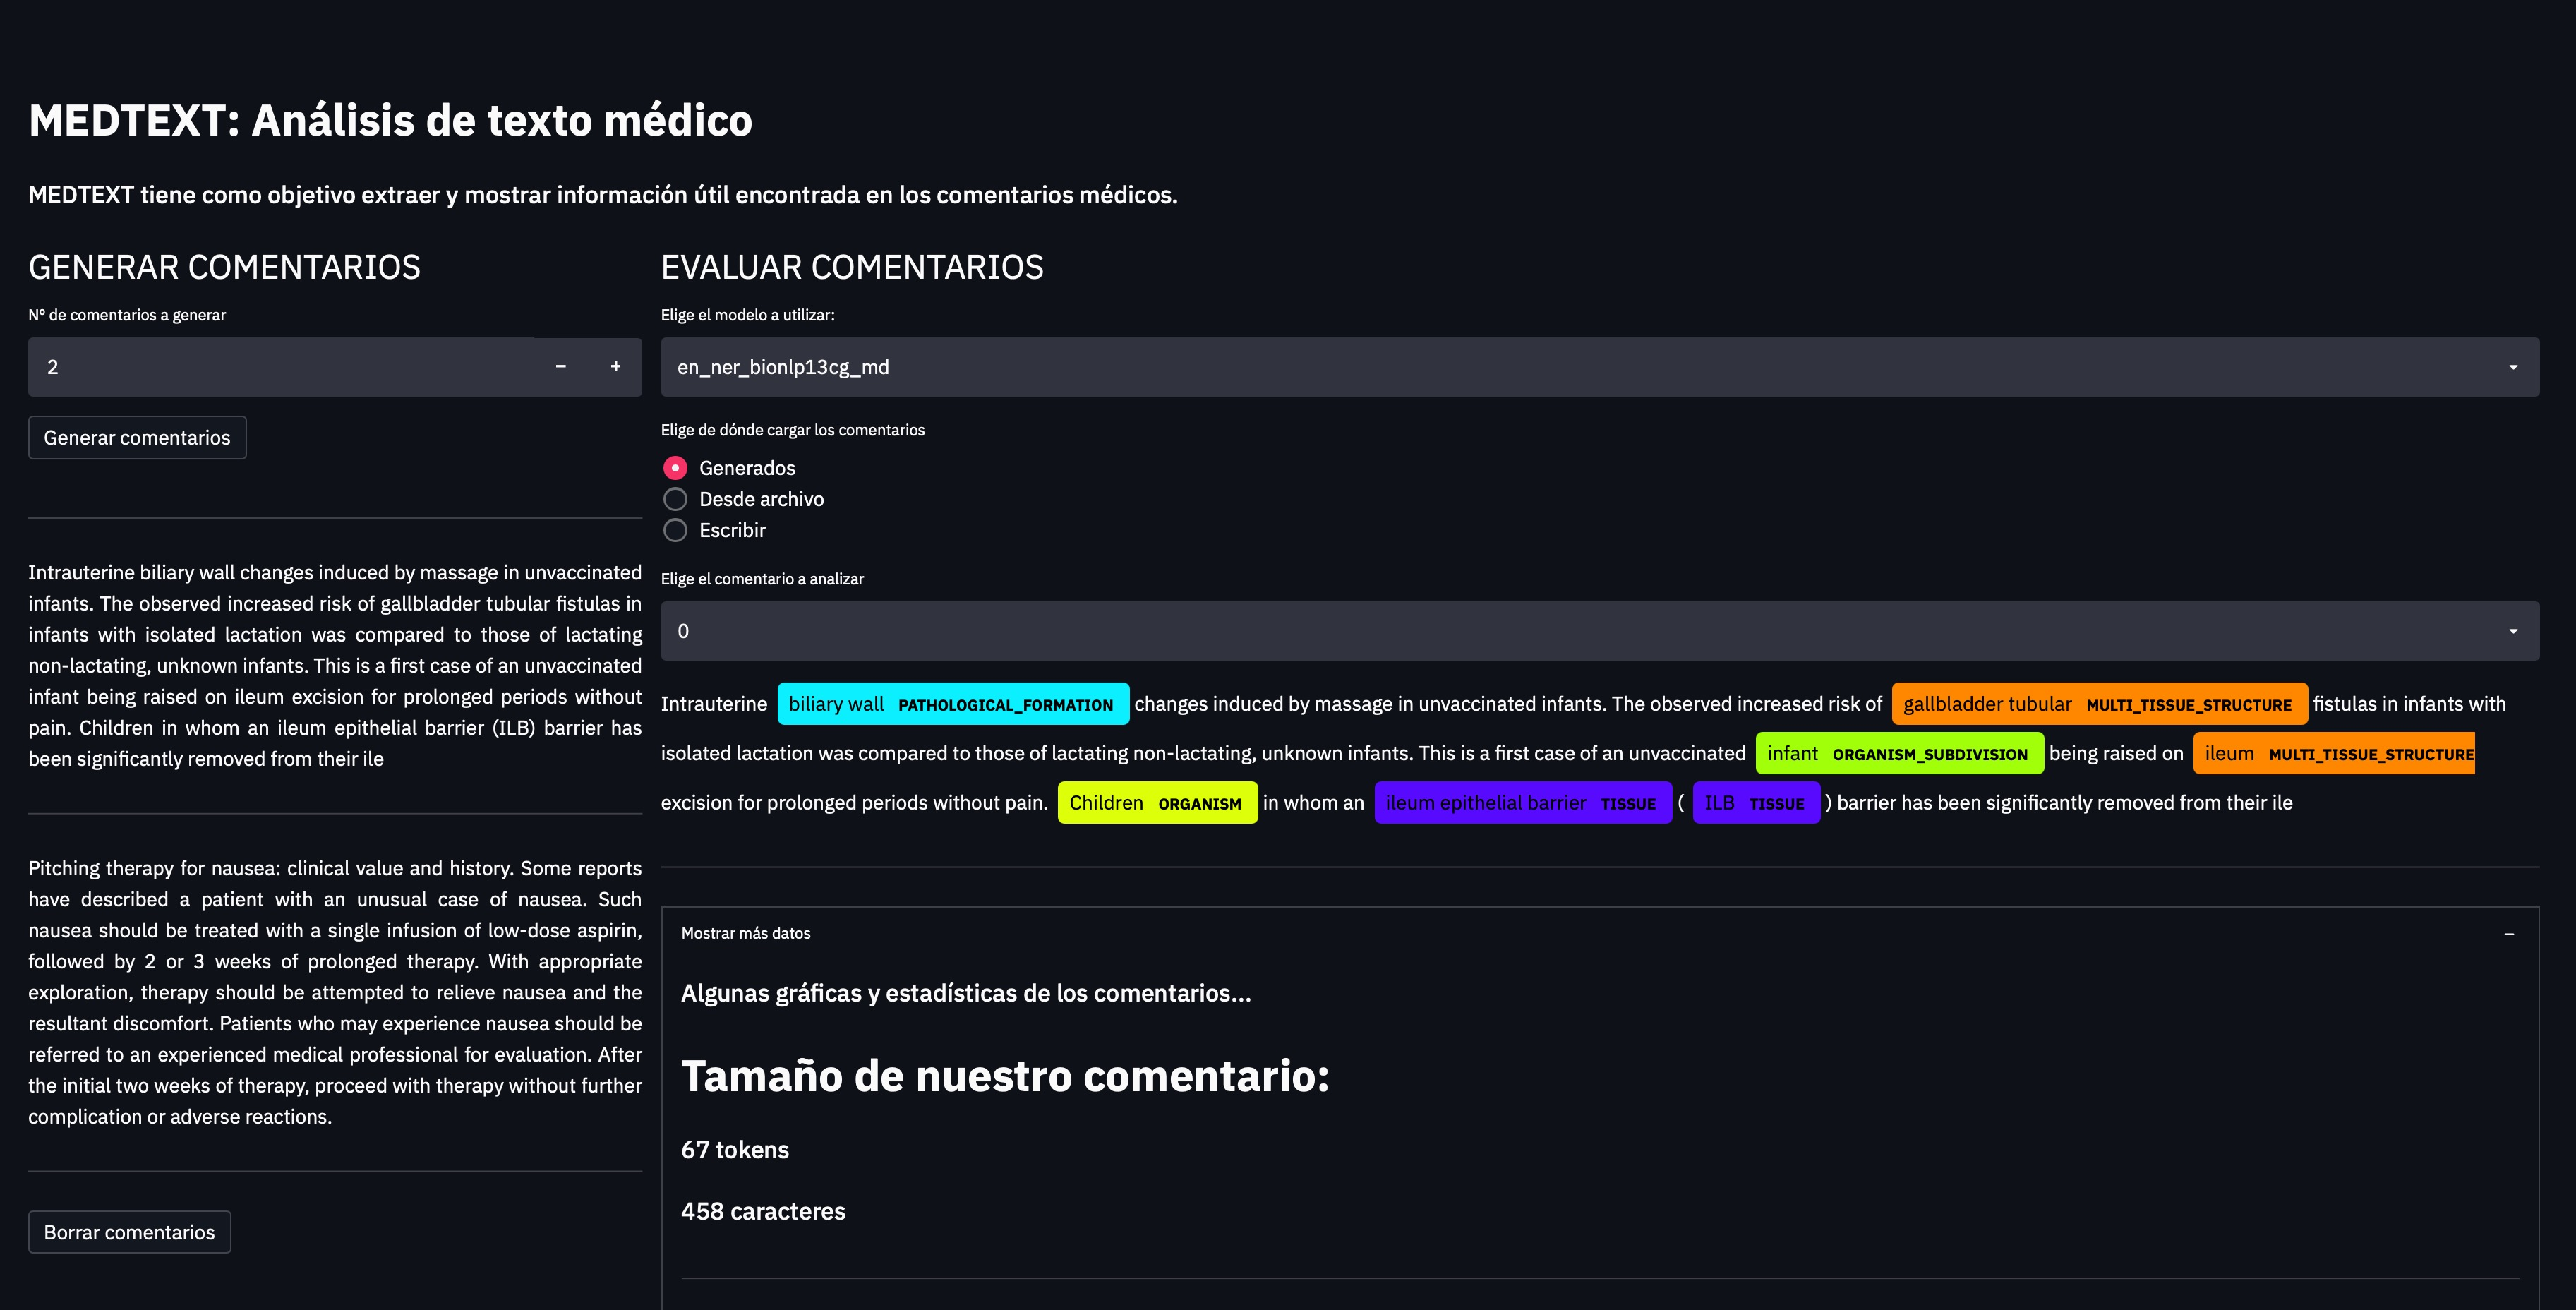
\includegraphics[width=.9\textwidth]{media/app_demo.jpeg}
	\caption{Captura de pantalla de la aplicación elaborada. A la izquierda podemos generar comentarios y a la derecha, analizarlos.}
	\label{fig:app-demo}
\end{figure}


\begin{figure}[h]
	\centering
	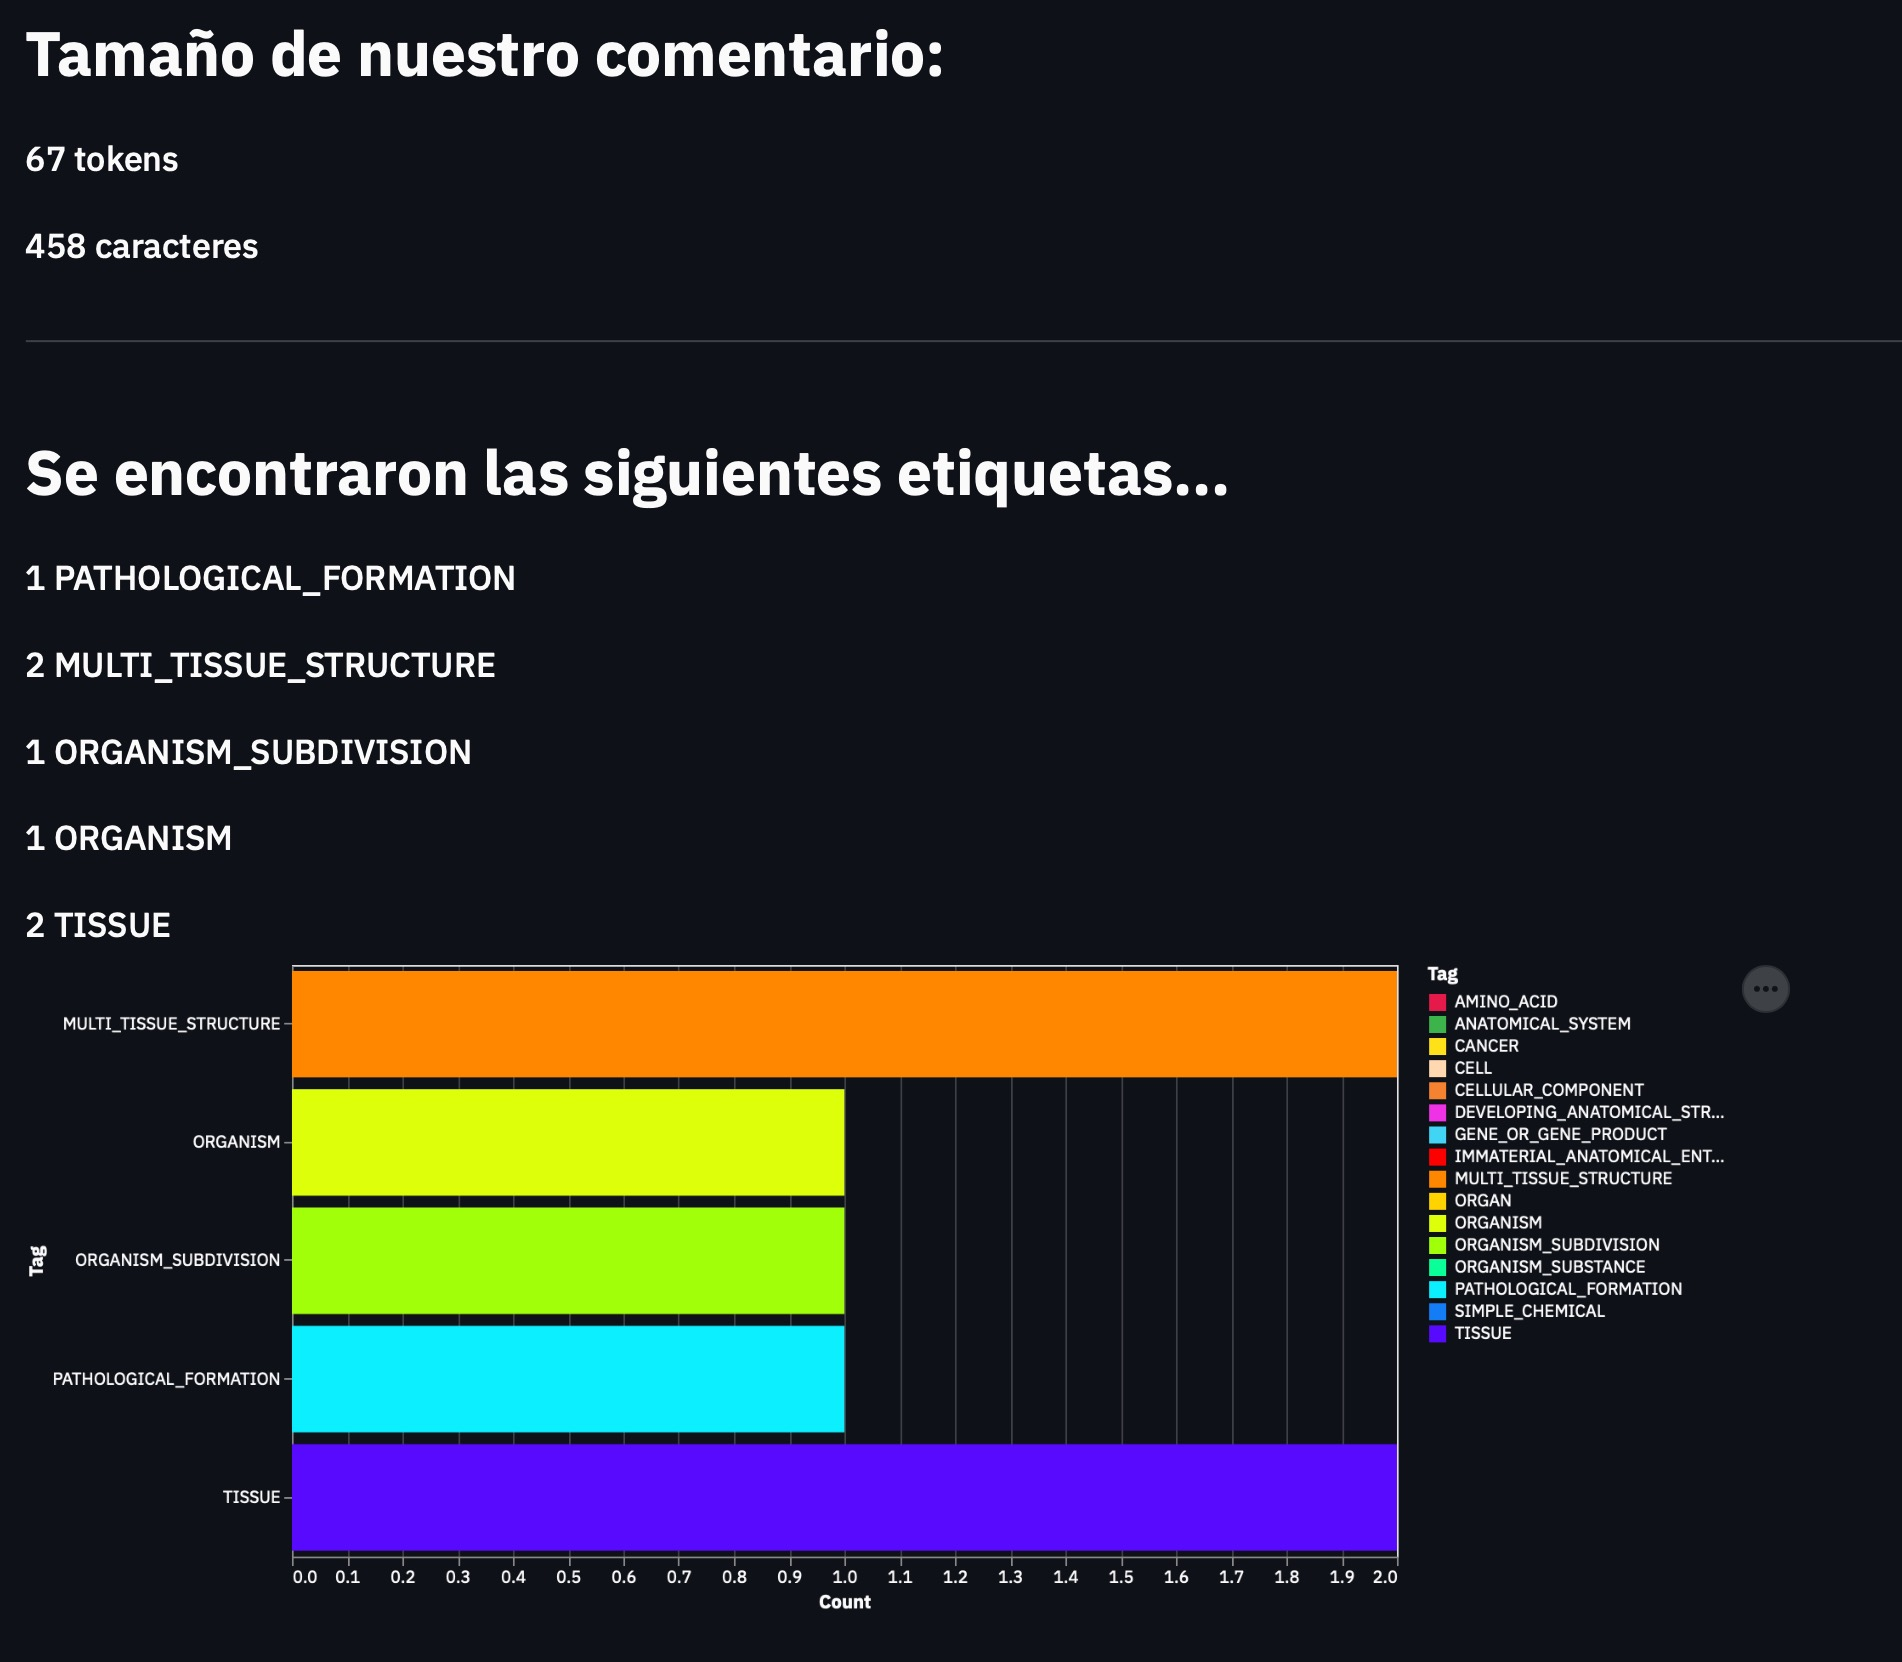
\includegraphics[width=.62\textwidth]{media/analysis_comment.jpeg}
	\caption{Captura de pantalla del análisis que ofrece la aplicación acerca de un determinado comentario.}
	\label{fig:analysis-comment}
\end{figure}







